\setcounter{secnumdepth}{1}

\chapter{Lab 3}


\begin{Task}{Question 3.1. Length data records}
    The FFT algorithm works faster when the length of the data records N is a power of 2. Do you know why?
\end{Task}

To numerically implement a DFT, the DFT algorithm is used. It works by dividing the input signal into two parts, each of which is transformed separately, and then the results are combined and this is done recursively. It means that a number of samples that is a power of 2 will be perfectly divided at each step, leading to a faster computation.

\begin{Task}{Question 3.2. Trigger signal}
    What is the purpose of a trigger signal? A number of processing methods were discussed in the theory to improve the SNR of the FRF by averaging of measurements. Which methods require a trigger signal to operate properly? Explain what happens if the trigger is absent while needed.
\end{Task}

For the averaging in the time domain and the averaging in the DFT spectra, the input and output signals need to be identical:
\begin{align*}
    H_{\text{time}}(j\omega_k) = \frac{\textbf{DFT}\left(\frac{1}{M}\sum_{i=1}^{M}y_i(n)\right)}{\textbf{DFT}\left(\frac{1}{M}\sum_{i=1}^{M}u_i(n)\right)}\\
    H_{\text{DFT}}(j\omega_k) = \frac{\frac{1}{M}\sum_{i=1}^{M}\textbf{DFT}\left(y_i(n)\right)}{\frac{1}{M}\sum_{i=1}^{M}\textbf{DFT}\left(u_i(n)\right)}
\end{align*}

For the measurements to be identical between two repetitions (except for the noise of course), they should always start at the same point in the period of the excitation and the trigger signal make sure it is the case.

\begin{Task}{Question 3.3. Frequency domain multisine}
    In your report, show the Matlab code you used to construct the multisine signal (with random or Schroeder phase) in the frequency domain. Make sure that the code is sufficiently commented to improve its readability.
\end{Task}

\begin{lstlisting}[language=Matlab, basicstyle=\ttfamily\footnotesize, keywordstyle=\color{blue}, commentstyle=\color{darkerGreen}, stringstyle=\color{red}]
    fs = 16000;                 % Sampling frequency
    excFreq = [4 1000];         % Excited frequencies in Hz
    rmsVal = 0.5;               % RMS value
    N = 4000;                   % Number of samples
    
    m = (excFreq(1)*N/fs:excFreq(2)*N/fs); 
                                % Excited frequencies in bins
    K = length(m);              % Number of excited frequencies
    
    shroedPhase = m.*(m+1) * pi / K;
    signalFreq = zeros(1, N);
    
    signalFreq(m + 1) = exp(1j*shroedPhase);
                                % m + 1 because the index starts from 1 in MATLAB
    
                                % Generate the signal
    signalTime = 2*N*real(ifft(signalFreq)); 
                                % Normalize the signal
    signalTime = signalTime*rmsVal/rms(signalTime); 
\end{lstlisting}


\begin{Task}{Question 3.4. Averaging the measurements}
    Which averaging techniques are applicable to which excitation signals? Explain.
\end{Task}

The time averaging and the frequency averaging can be applied with the periodic excitation only. The issue with a random input is that averaging it could still result in some bins with a close to zero amplitude, wich would create spikes in the FRF. It is worth noting that these two methods are equivalent (at least theoretically, in practice there are some differences due to the way they are implemented).\\

Computing the FRF of each repetition separately and then averaging them could also lead to a division by zero, making it unusable for the random excitation.\\

Finally, using the average of the auto-power of the input/output is a method that can be used for any input signal as it divides by a power that is not zero. It is preferred to use the average of the auto-power of the input signal as it is less noisy than the output signal. This is because de DUT is a filter and the output signal is lower in amplitude than the input signal, leading to a smaller SNR. It must be noted that these methods introduce a bias. This bias however is null if the additive noise is circular complex.
\normalsize

\begin{Task}{Question 3.5. Plots}
    Provide relevant plots of the estimated FRF, obtained with the different methods, with the different excitation signals and with a different number of averaged records.
\end{Task}

On the 3 first figures, the aperiodic FRF is "too clean". It should have more spikes as explained in question 3.4.

\begin{figure}[H]
    \centering
    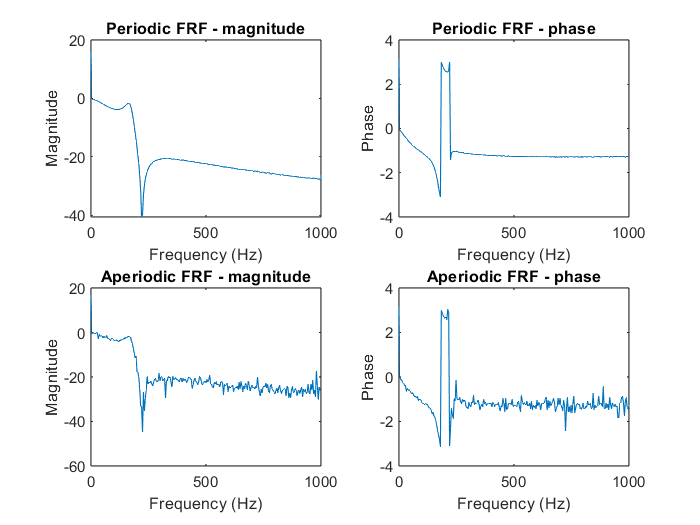
\includegraphics[width=0.8\textwidth]{part3/time_avg.png}
    \caption{Estimated FRF with time averaging}
\end{figure}

\begin{figure}[H]
    \centering
    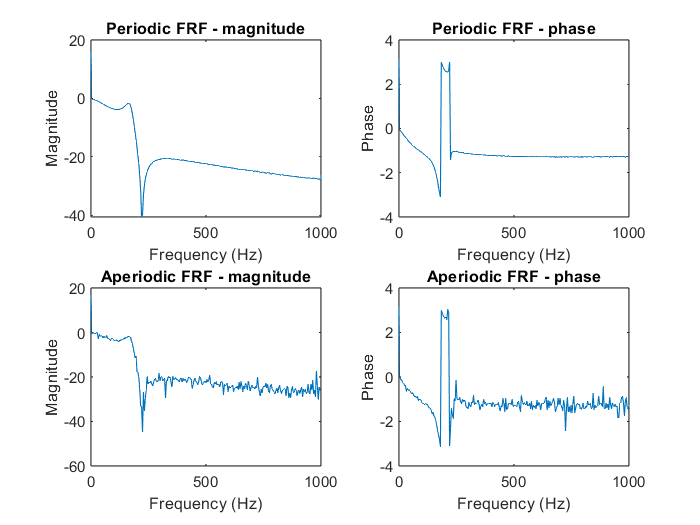
\includegraphics[width=0.8\textwidth]{part3/dft_avg.png}
    \caption{Estimated FRF with frequency averaging}
\end{figure}

\begin{figure}[H]
    \centering
    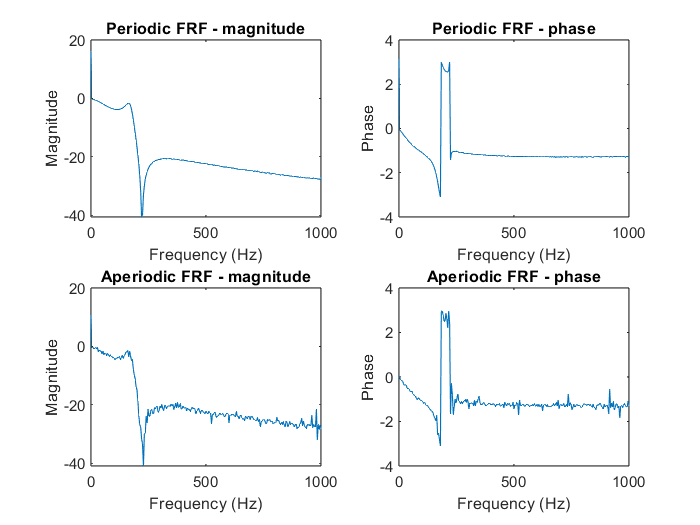
\includegraphics[width=0.8\textwidth]{part3/frf_avg.png}
    \caption{Estimated FRF by averaging the FRF}
\end{figure}

\begin{figure}[H]
    \centering
    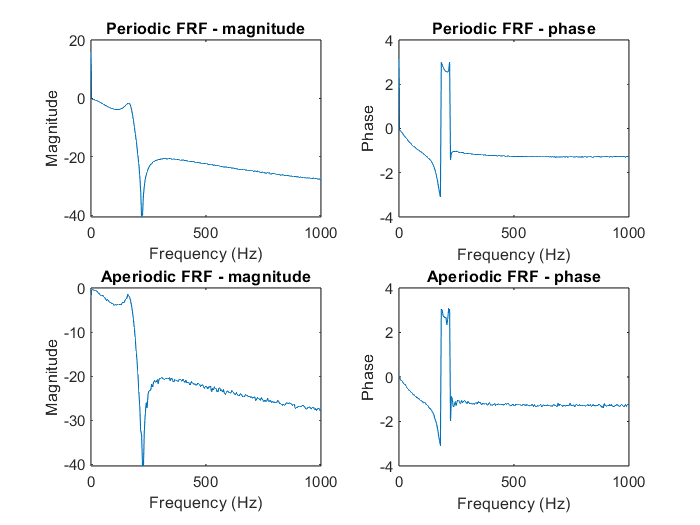
\includegraphics[width=0.8\textwidth]{part3/input_power.png}
    \caption{Estimated FRF by averaging the auto-power of the input signal}
\end{figure}

\begin{figure}[H]
    \centering
    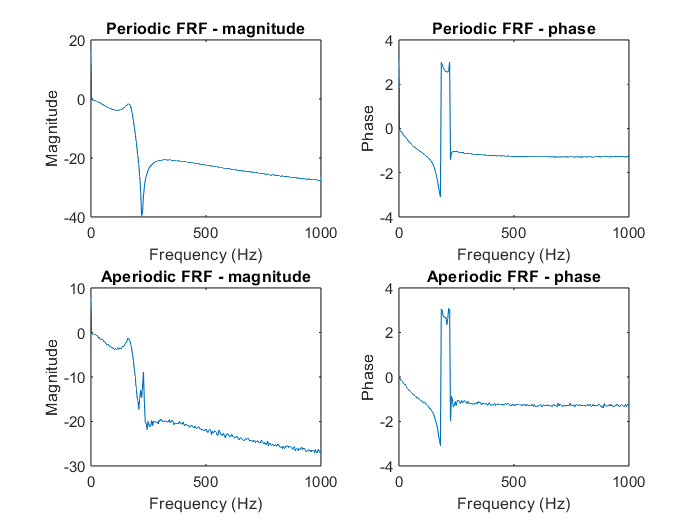
\includegraphics[width=0.8\textwidth]{part3/output_power.png}
    \caption{Estimated FRF by averaging the auto-power of the output signal}
\end{figure}

Here is the effect of the number of averaged records for the time averaging method:

\begin{figure}[H]
    \centering
    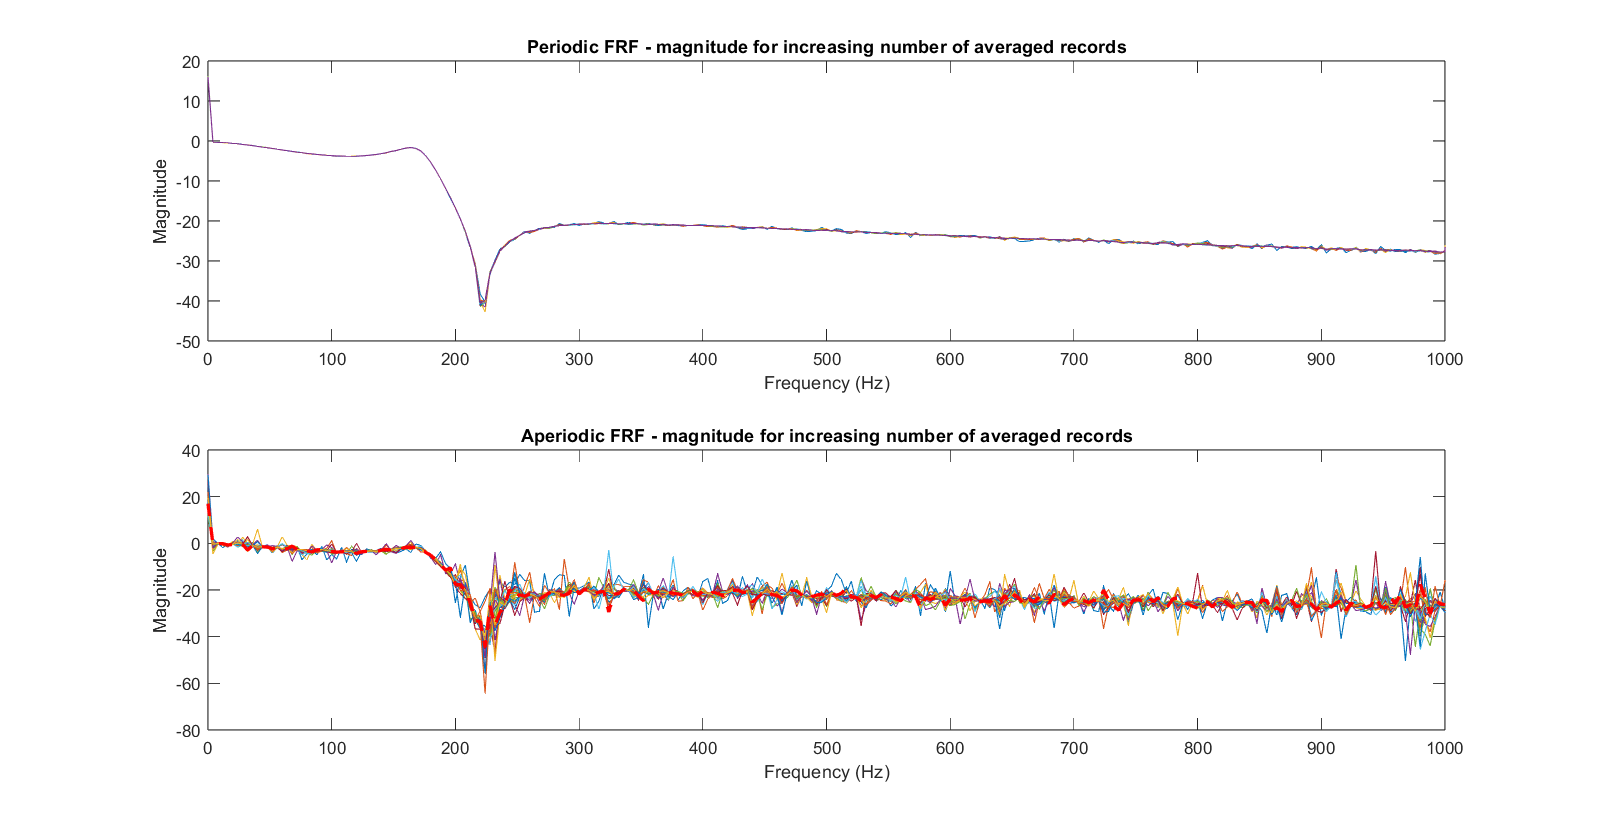
\includegraphics[width=0.8\textwidth]{part3/increasingAveragedRecords.png}
    \caption{Estimated FRF for different number of averaged records}
\end{figure}

Because the transient has been removed by discarding the first 8 periods, the estimated FRF based on the periodic signal does not change. This indicates that the noise power was extremely small compared to the signal power (we might have accidentally saved the response of a noiseless test). The estimated FRF based on the random input is however more interesting: the last estimation (the red dotted line) has way less spikes than all the previous ones. It really shows the benefit of averaging the measurements.

\begin{Task}{Question 3.6. Impact of repetition number}
    Determine the effect of the number of averaged records on the variability of the averaged result. Compare the standard deviation.
\end{Task}

\huge{TODO}
\normalsize

\begin{Task}{Question 3.7. Discussion}
    Discuss the differences and explain according to you, which will deliver the best result. Discuss the pros and cons of each excitation signal.
\end{Task}

\huge{TODO}
\normalsize
